% e-puck IR field-of-view diagram (left: IR6+IR7, right: IR0+IR1)
% Units: mm (matches robot geometry: body diameter 70, FOV radius 55)
\documentclass[tikz,border=10pt]{standalone}
\begin{document}
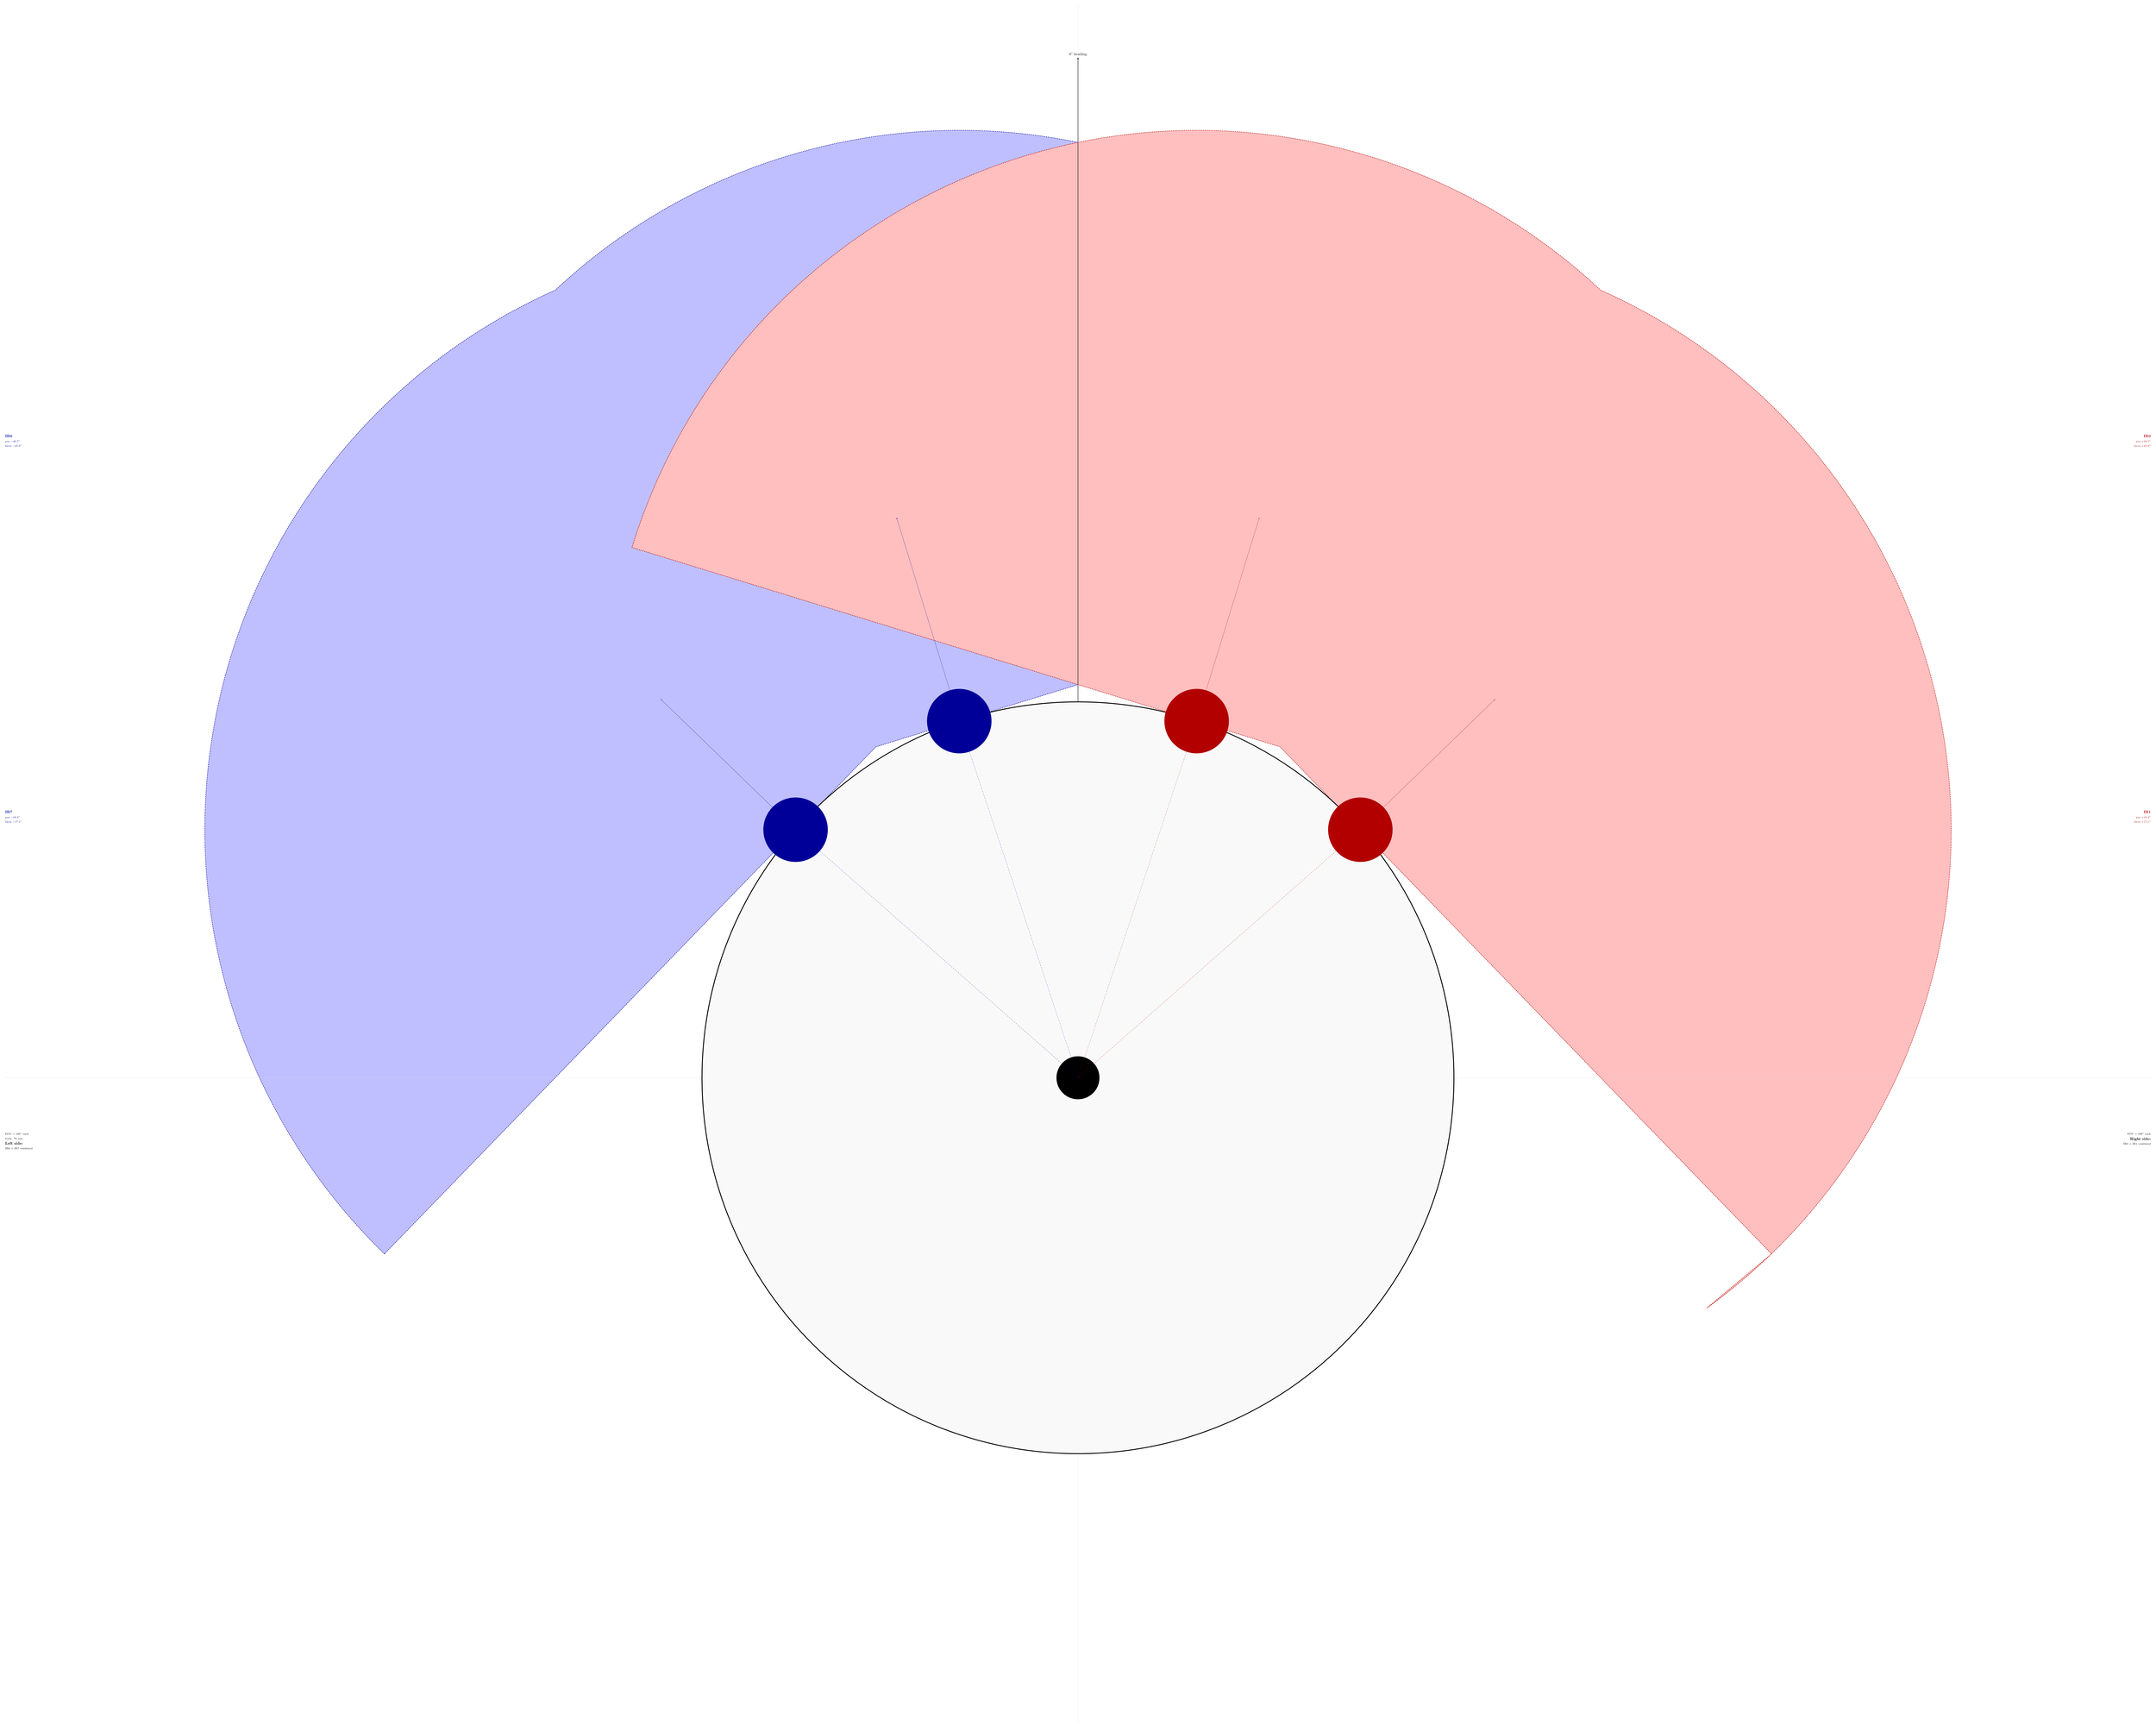
\begin{tikzpicture}[>=stealth,
  lbl/.style={font=\small},
  sub/.style={font=\scriptsize}]

  % ---- combined FOV regions (union of two 180-deg wedges each) ----
  % Left side (IR6 + IR7), light blue
  \filldraw[fill=blue!25, draw=blue!60!black, dash pattern=on 3pt off 2pt, line width=0.4mm]
    (-64.57,-16.40)
    -- (-26.29,23.10)            % IR6 mount
    -- (-18.81,30.82)            % edge ray enters IR7 coverage
    -- (-11.05,33.21)            % IR7 mount
    -- (41.52,49.38)
    arc[start angle=17.10, end angle=133.13, radius=55]   % around IR7, through its tip
    arc[start angle=113.99, end angle=225.90, radius=55]   % around IR6, through its tip
    -- cycle;

  % Right side (IR0 + IR1), light red (mirror image)
  \filldraw[fill=red!25, draw=red!70!black, dash pattern=on 3pt off 2pt, line width=0.4mm]
    (64.57,-16.40)
    -- (26.29,23.10)             % IR0 mount
    -- (18.81,30.82)             % edge ray enters IR1 coverage
    -- (11.05,33.21)             % IR1 mount
    -- (-41.52,49.38)
    arc[start angle=162.90, end angle=46.87, radius=55]    % around IR1, through its tip
    arc[start angle=66.01, end angle=-54.10, radius=55]   % around IR0, through its tip
    -- cycle;

  % ---- grid / axes ----
  \draw[gray!30] (-100,0) -- (100,0);
  \draw[gray!30] (0,-60) -- (0,100);

  % ---- robot body: circle, 70 mm diameter ----
  \draw[line width=0.8mm, fill=gray!5] (0,0) circle (35);
  \fill (0,0) circle (2);

  % ---- heading reference (0 deg) ----
  \draw[->, line width=0.4mm] (0,35) -- (0,95)
      node[above, black] {$0^\circ$ heading};

  % ---- position rays (mount angles from center) ----
  \draw[blue!60!black, dashed, thin] (0,0) -- (-26.29,23.10);
  \draw[blue!60!black, dashed, thin] (0,0) -- (-11.05,33.21);
  \draw[red!70!black, dashed, thin] (0,0) -- (26.29,23.10);
  \draw[red!70!black, dashed, thin] (0,0) -- (11.05,33.21);

  % ---- facing direction arrows ----
  \draw[->, blue!60!black] (-26.29,23.10) -- (-38.84,35.25);
  \draw[->, blue!60!black] (-11.05,33.21) -- (-16.88,52.14);
  \draw[->, red!70!black]   (26.29,23.10) -- (38.84,35.25);
  \draw[->, red!70!black]   (11.05,33.21) -- (16.88,52.14);

  % ---- sensor mount points ----
  \fill[blue!60!black] (-26.29,23.10) circle (3);
  \fill[blue!60!black] (-11.05,33.21) circle (3);
  \fill[red!70!black]   (26.29,23.10) circle (3);
  \fill[red!70!black]   (11.05,33.21) circle (3);

  % ---- labels: left ----
  \node[align=left, anchor=north west] at (-100,60)
    {\textcolor{blue!60!black}{\textbf{IR6}}\\[1pt]
     \textcolor{blue!60!black}{\scriptsize pos $-48.7^\circ$}\\
     \textcolor{blue!60!black}{\scriptsize faces $-45.9^\circ$}};
  \node[align=left, anchor=north west] at (-100,25)
    {\textcolor{blue!60!black}{\textbf{IR7}}\\[1pt]
     \textcolor{blue!60!black}{\scriptsize pos $-18.4^\circ$}\\
     \textcolor{blue!60!black}{\scriptsize faces $-17.1^\circ$}};
  \node[align=left, anchor=north west, text=black] at (-100,-5)
    {\scriptsize FOV $=180^\circ$ each\\ \scriptsize body $\varnothing$ 70 mm\\[2pt]
     \textbf{Left side:}\\ \scriptsize IR6 + IR7 combined};

  % ---- labels: right ----
  \node[align=right, anchor=north east] at (100,60)
    {\textcolor{red!70!black}{\textbf{IR0}}\\[1pt]
     \textcolor{red!70!black}{\scriptsize pos $+48.7^\circ$}\\
     \textcolor{red!70!black}{\scriptsize faces $+45.9^\circ$}};
  \node[align=right, anchor=north east] at (100,25)
    {\textcolor{red!70!black}{\textbf{IR1}}\\[1pt]
     \textcolor{red!70!black}{\scriptsize pos $+18.4^\circ$}\\
     \textcolor{red!70!black}{\scriptsize faces $+17.1^\circ$}};
  \node[align=right, anchor=north east, text=black] at (100,-5)
    {\scriptsize FOV $=180^\circ$ each\\[2pt]
     \textbf{Right side:}\\ \scriptsize IR0 + IR1 combined};

\end{tikzpicture}
\end{document}
